%        File: symmetries-and-polynomials-notes.tex
%     Created: Thu May 17 10:00 AM 2018 P
% Last Change: Thu May 17 10:00 AM 2018 P
%
%%%%%%%%%%%%%%%%%%%%%
%   AMS packages    %
%%%%%%%%%%%%%%%%%%%%%
% \documentclass[12 pt, reqno]{amsart}

\documentclass[reqno, 12pt, letter]{article}
\usepackage[margin=1in]{geometry}
\usepackage{mdframed}

\usepackage{hyperref}
\usepackage{etex}
\usepackage[shortlabels]{enumitem}
\usepackage{amsmath}
\usepackage{amsxtra}
\usepackage{amscd}
\usepackage{amsthm}
\usepackage{amsfonts}
\usepackage{amssymb}
\usepackage{eucal}
\usepackage[all]{xy}
\usepackage{graphicx}
\usepackage{tikz-cd}
\usepackage{mathrsfs}
\usepackage{subfiles}
\usepackage{mathpazo}
%\usepackage{euler}
\usepackage[colorinlistoftodos, textsize=tiny]{todonotes}
\usepackage{morefloats}
\usepackage{pdfpages}
\usepackage{thm-restate}
\usepackage[utf8]{inputenc}
\usepackage{epigraph}
\usepackage{csquotes}
\usepackage{gensymb}
% \usepackage[margin=1.5in]{geometry}

\graphicspath{ {images/} }

\RequirePackage{color}
\definecolor{myred}{rgb}{0.75,0,0}
\definecolor{mygreen}{rgb}{0,0.5,0}
\definecolor{myblue}{rgb}{0,0,0.65}

\usepackage{hyperref}
\hypersetup{citecolor=blue}
\usepackage{tikz}
\usetikzlibrary{matrix,arrows,decorations.pathmorphing}

\theoremstyle{plain}
\newtheorem{theorem}{Theorem}[section]
\newtheorem{proposition}[theorem]{Proposition}
\newtheorem{lemma}[theorem]{Lemma}
\newtheorem{corollary}[theorem]{Corollary}
\theoremstyle{definition}
\newtheorem{definition}[theorem]{Definition}
\newtheorem{remark}[theorem]{Remark}
\newtheorem{example}[theorem]{Example}
\newtheorem{exercise}[theorem]{Exercise}
\newtheorem{counterexample}[theorem]{Counterexample}
\newtheorem{convention}[theorem]{Convention}
\newtheorem{question}[theorem]{Question}
\newtheorem{conjecture}[theorem]{Conjecture}
\newtheorem{goal}[theorem]{Goal}
\newtheorem{warn}[theorem]{Warning}
\newtheorem{fact}[theorem]{Fact}
\theoremstyle{remark}
\newtheorem{notation}[theorem]{Notation}
\numberwithin{equation}{section}

\newcommand\nc{\newcommand}
\nc\on{\operatorname}
\nc\renc{\renewcommand}
\newcommand\se{\section}
\newcommand\ssec{\subsection}
\newcommand\sssec{\subsubsection}
\newcommand\bn{{\mathbb N}}
\newcommand\bc{{\mathbb C}}
\newcommand\br{{\mathbb R}}
\newcommand\bq{{\mathbb Q}}
\newcommand\bp{{\mathbb P}}
\newcommand\CF{{\mathscr F}}
\newcommand\bz{{\mathbb Z}}
\newcommand\ba{{\mathbb A}}
\newcommand\bg{{\mathbb G}}
\newcommand\fa{{\mathfrak a}}
\newcommand\fp{{\mathfrak p}}
\newcommand\fq{{\mathfrak q}}
\newcommand\fm{{\mathfrak m}}
\newcommand\fg{{\mathfrak g}}
\newcommand\fh{{\mathfrak h}}
\newcommand\fgl{{\mathfrak {gl}}}
\newcommand\fsu{{\mathfrak {su}}}
\newcommand\fsl{{\mathfrak {sl}}}
\newcommand\fso{{\mathfrak {so}}}
\newcommand\fo{{\mathfrak {o}}}
\newcommand\fu{{\mathfrak {u}}}
\newcommand\fsp{{\mathfrak {sp}}}
\newcommand\fgsp{{\mathfrak {gsp}}}



\newcommand\sca{\mathscr A}
\newcommand\scb{\mathscr B}
\newcommand\scc{\mathscr C}
\newcommand\scd{\mathscr D}
\newcommand\sce{\mathscr E}
\newcommand\scf{\mathscr F}
\newcommand\scg{\mathscr G}
\newcommand\sch{\mathscr H}
\newcommand\sci{\mathscr I}
\newcommand\scj{\mathscr J}
\newcommand\sck{\mathscr K}
\newcommand\scl{\mathscr L}
\newcommand\scm{\mathscr M}
\newcommand\scn{\mathscr N}
\newcommand\sco{\mathscr O}
\newcommand\scp{\mathscr P}
\newcommand\scq{\mathscr Q}
\newcommand\scs{\mathscr S}
\newcommand\sct{\mathscr T}
\newcommand\scu{\mathscr U}
\newcommand\scv{\mathscr V}
\newcommand\scw{\mathscr W}
\newcommand\scx{\mathscr X}
\newcommand\scy{\mathscr Y}
\newcommand\scz{\mathscr Z}

\newcommand \ra{\rightarrow}
\newcommand \xra{\xrightarrow}
\DeclareMathOperator\spec{\text{Spec }}
\DeclareMathOperator\proj{\text{Proj }}
\DeclareMathOperator\rspec{\textit{Spec }}
\DeclareMathOperator\rproj{\textit{Proj }}
\newcommand*{\shom}{\mathscr{H}\kern -.5pt om}
\newcommand*{\stor}{\mathscr{T}\kern -.5pt or}
\newcommand*{\sext}{\mathscr{E}\kern -.5pt xt}
\newcommand \mg{{\mathscr M_g}}

\makeatletter
\newcommand{\customlabel}[2]{\protected@write \@auxout {}{\string \newlabel {#1}{{#2}{\thepage}{#2}{#1}{}} }\hypertarget{#1}{#2}}
\newcommand\sh[1]{\sco_{#1}^{\rm{sh}}}
\DeclareMathOperator\id{id}
\DeclareMathOperator\tor{Tor}
\renewcommand\hom{Hom}
\DeclareMathOperator\coker{coker}
\DeclareMathOperator\ord{ord}
\DeclareMathOperator\hilb{Hilb}
\DeclareMathOperator\rk{rk}
\DeclareMathOperator\di{div}
\DeclareMathOperator\pic{Pic}
\DeclareMathOperator\lcm{lcm}
\DeclareMathOperator\rank{rank}
\DeclareMathOperator\codim{codim}
\DeclareMathOperator\vol{Vol}
\DeclareMathOperator\supp{Supp}
\DeclareMathOperator\spn{Span}
\DeclareMathOperator\im{im}
\DeclareMathOperator\End{End}
\DeclareMathOperator\sym{Sym}
\DeclareMathOperator\pgl{PGL}
\DeclareMathOperator\sat{Sat}
\DeclareMathOperator\blow{Bl}
\renewcommand\sp{\mathrm{Sp}}
\DeclareMathOperator\gsp{GSp}
\DeclareMathOperator\sgn{sgn}
\DeclareMathOperator\gal{gal}
\DeclareMathOperator\tr{tr}
\renewcommand\char{char}
\newcommand\bbf{{\mathbb F}}
\newcommand\bk{{\Bbbk}}
\newcommand\ul{\underline}
\newcommand\ol{\overline}
\DeclareMathOperator\pr{pr}
\DeclareMathOperator\ev{ev}
\DeclareMathOperator\maj{maj}
\DeclareMathOperator\inv{inv}
\DeclareMathOperator\isom{isom}
\DeclareMathOperator\mor{mor}
\DeclareMathOperator\aut{Aut}
\DeclareMathOperator\gl{GL}
\renewcommand\sl{\mathrm{SL}}
\DeclareMathOperator\mat{Mat}
\DeclareMathOperator\stab{Stab}
\DeclareMathOperator\so{SO}
\DeclareMathOperator\su{SU}
\renewcommand\u{\mathrm{U}}
\DeclareMathOperator\lie{Lie}
\DeclareMathOperator\ad{ad}
\DeclareMathOperator\Ad{Ad}
\renewcommand\o{{\rm{O}}}

\renewcommand{\thefootnote}{\fnsymbol{footnote}}
%\newcommand{\hint}[1]{\footnote{\raggedleft\rotatebox{180}{\tiny{{Hint:} #1\hfill}}}}
\newcommand{\hint}[1]{\footnote{{Hint:} #1\hfill}}


\setcounter{MaxMatrixCols}{20}

\def\listtodoname{List of Todos}
\def\listoftodos{\@starttoc{tdo}\listtodoname}

\usepackage{endnotes}

\let\footnote=\endnote



\title{Symmetries and Polynomials}
\author{Aaron Landesman and Apurva Nakade}

\usepackage{microtype}
\begin{document}

\maketitle


\section*{Introduction}
In this class we'll learn how to solve a cubic. We'll also sketch how to solve a quartic. We'll explore the connections between these solutions and group theory.
Towards the end, we'll hint towards the deep connection between polynomials and groups via Galois Theory. This connection allows one to convert the classical question of whether a general quintic can be solved by radicals to a group theory problem, which can be relatively easily answered.

The 5 day outline is as follows:
\begin{enumerate}
	\item The first two days are dedicated to studying polynomials. On the first day, we'll study a simple invariant associated to every polynomial, the discriminant.
	\item On the second day, we'll solve the cubic equation by a method motivated by Galois theory.
	\item Days $3$ and $4$ are a ``practical'' introduction to group theory. On day $3$ we'll learn about groups as symmetries of geometric objects.
	\item On day $4$, we'll learn about the commutator subgroup of a group.
	\item Finally, on the last day we'll connect the two theories and explain the Galois correspondence for the cubic and the quartic.
\end{enumerate}
There are plenty of optional problems along the way for those who wish to explore more.
Tricky optional problems are marked with $*$, and especially tricky optional problems are marked with $**$.

\newpage
\section{The Discriminant}
Today we'll introduce the discriminant of a polynomial. The discriminant of a polynomial $P$ is another polynomial $Q$ which tells you
whether $P$ has any repeated roots over $\bc$.

\subsection{Quadratic Polynomials}
\begin{definition}[Quadratic discriminant]
	\label{definition:quadratic-discriminant}
	Let $P(x) = x^2 + bx + c$ be a polynomial with $b$ and $c$ real numbers.
	The discriminant $\Delta(P)$ is by definition $b^2 - 4c$.
\end{definition}
\begin{exercise}
	\label{exercise:}
	If the polynomial $P(x) = x^2 + bx + c$ has roots $\alpha$ and $\beta$, express $b$ and $c$
	in terms of $\alpha$ and $\beta$.
\end{exercise}
\begin{exercise}
	\label{exercise:quadratic-roots}
	What does the sign of the discriminant (i.e., whether $\Delta(P) > 0, < 0$ or $=0$)
	tell you about the roots $\alpha$ and $\beta$?
	\footnote{{\it Hint:} If the discriminant is $>0$ show that the roots are real, if it is equal
		to $0$, show they are the same, if it is less than $0$, show they are complex numbers
		which are not real.}
\end{exercise}
\begin{exercise}
	\label{exercise:quadratic-discriminant-in-roots}
	Express the discriminant of the polynomial $P(x) = x^2 + bx + c$ in terms of
	the roots $\alpha$ and $\beta$.
\end{exercise}

\subsection{The discriminant in general}
\begin{definition}
	\label{definition:discriminant}
	For $P(x)$ a polynomial of the form $P(x) = (x-r_1)(x-r_2) \cdots (x-r_n)$,
	define the discriminant $\Delta(P) := \prod_{1 \leq i < j \leq n} (r_i - r_j)^2$.
\end{definition}
\begin{exercise}
	\label{exercise:}
	Verify that for $P(x)$ of degree $2$, the definition of the discriminant
	of a general polynomial from \autoref{definition:discriminant} agrees with
	that of a quadratic polynomial given in \autoref{definition:quadratic-discriminant}.
	\footnote{{\it Hint:} Use \autoref{exercise:quadratic-discriminant-in-roots}.}
\end{exercise}
\begin{exercise}
	\label{exercise:discriminant-vanishing}
	Show that for $P$ a polynomial, $\Delta(P) = 0$ if and only if $P$ has a repeated root over $\bc$.
\end{exercise}
\subsection{Cubic discriminants}
\begin{exercise}
	\label{exercise:real-root-cubic}
	Show that a cubic polynomial $P(x) := x^3 + ax + bx + c$
	with real coefficients 	always has a real root.
	\footnote{{\it Hint:} Graph the cubic and show it intersects the line $P(x) = 0$.}
\end{exercise}
\begin{exercise}
	\label{exercise:}
	Using \autoref{exercise:real-root-cubic}, show that a cubic polynomial either has
	\begin{enumerate}
		\item $3$ real roots or
		\item $2$ complex conjugates roots (of the form $a + bi, a-bi$ for $a,b$ real numbers) and one real root.
		      \footnote{{\it Hint:} Factor out the real root, and use your understanding of quadratic polynomials.}
	\end{enumerate}
\end{exercise}
\begin{exercise}
	\label{exercise:discriminant-cubic-sign}
	For $P(x) = x^3 + ax^2 + bx + c$ a cubic polynomial with real coefficients, show $\Delta(P) = 0$ if and only
	if there is a repeated root over $\bc$, $\Delta(P) > 0$ if and only if $P$ has three distinct real roots, and $\Delta(P) < 0$ if and only if $P$ has two complex conjugate roots and one real root.
	Compare your answer to \autoref{exercise:quadratic-roots}.
\end{exercise}

{\it Your homework is to complete up through \autoref{exercise:discriminant-cubic-sign}. If you finish that, and still have time try the following questions.}

\subsection{Further optional questions on discriminants}

\begin{exercise}[Optional 1]
	\label{exercise:cubic-discriminant}
	An amazing fact about the discriminant is that it can always be written as a polynomial in terms of the coefficients. For the quadratic this was shown in \autoref{definition:quadratic-discriminant} and \autoref{exercise:quadratic-discriminant-in-roots}. Now let's see this for a \textbf{depressed cubic} (i.e. a cubic with coefficient of $ x^2$ equal to $0$). Consider the cubic
	\begin{align*}
		P(x) & = x^3 + px + q.
	\end{align*}
	Assume that not all three roots are the same.
	\begin{enumerate}
		\item By definition, the {\bf critical points} of $P(x)$
		      %	(the points at which $ P(x)$ attains its local max/min if at all)
		      are roots of $P'(x) = 3x^2 + p$. Find the critical points of $ P(x)$, and call them $ x_1, x_2$.
		\item Show that $ P(x_1) \cdot P(x_2) = 4(p/3)^3 - q^2$.
		\item Argue that $ P(x)$ has a repeated root over $\bc$ if and only if $ P(x_1) \cdot P(x_2) = 0$.
	\end{enumerate}
	\begin{remark}
		This is very close to the statement that $\Delta(P) = 0$ iff $P(x)$ has a repeated root, which is not coincidental. By a direct computation one can show that the discriminant of the cubic $ P(x)$ equals
		\begin{align*}
			\Delta(P) = -27P(x_1) \cdot P(x_2) = -4p^3 - 27q^2
		\end{align*}
	\end{remark}
\end{exercise}

\subsection{Counting polynomials of discriminant $0$}
The following questions are quite tricky, but fun. Only attempt them if you've already solved \autoref{exercise:cubic-discriminant}.
\begin{exercise}[Optional 2]**
	\label{exercise:repeated-roots}
	Let $P(x) = x^n + a_{n-1}x^{n-1} + \cdots + a_0$, where now the coefficients $a_i$ are
	in $\bz/p$ (i.e., take on values between $0$ and $p-1$), and the discriminant is
	also considered as a number in $\bz/p$. To make sense of discriminant, you may assume that
	every such polynomial factors uniquely as a product of irreducible polynomials with coefficients in $\bz/p$.
	Show there are $p^n$ such polynomials, and exactly
	$p^{n-1}$ of them have discriminant $0$.
	Conclude that the number of square-free polynomials of degree $n$ over $\bz/p$ is $p^n - p^{n-1}$.
	\footnote{{\it Hint:}
		You may assume that every such polynomial $p(x)$ can be written uniquely
		as $f(x)g(x)^2$,
		where $f(x)$ is square-free. (Here, $f$ and $g$ are polynomials with $\bz/p$ coefficients.)
		Then count the number of such polynomials with $\deg f = k$ by induction on $k$.}
\end{exercise}

\begin{exercise}[Optional 3]**
	\label{exercise:common-roots}
	Using a similar method to that of \autoref{exercise:repeated-roots},
	count the number of pairs of degree $n$ polynomials $(P,Q)$ for
	$P(x) = x^n + a_{n-1}x^{n-1} + \cdots + a_0$ and $Q(x) = x^n + b_{n-1}x^{n-1} + \cdots + b_0$
	with $a_i \in \bz/p, b_i \in \bz/p$ so that $P$ and $Q$ have no common irreducible factor.\todo{How does one do this problem without using the previous problem?}
\end{exercise}
\begin{remark}
	\label{remark:}
	If you did the two prior exercises \autoref{exercise:repeated-roots} and \autoref{exercise:common-roots} correctly, you may notice a striking similarity
	between the two answers. There is indeed a deeper connection, but the answer lies deep.
	Loosely speaking, if you take a polynomial $P(x)$ with no repeated factors, you can send it
	to the pair of polynomials $(P(x) + P'(x), P(x))$. Here $P'(x)$ denotes the derivative of $P(x)$.
	If $P(x) = \sum_i a_ix^i$ then $P'(x) = \sum_i  i \cdot a_i x^{i-1}$.
	\begin{exercise}
		\label{exercise:}
		Verify that the above indeed defines a map
		from the space of polynomials with no repeated factors to the
		space of pairs of polynomials with no common factors.
	\end{exercise}

	In some sense (which we do not explain) this map explains why the counts from
	\autoref{exercise:repeated-roots} and \autoref{exercise:common-roots} are so similar.
\end{remark}



\newpage
\section{Solving the Cubic}
In this section, we will discover a method to solve the cubic, motivated by Galois theory.

We'll continue working with with the \emph{depressed} cubic (the coefficient of $x^2$ is $0$)
\begin{align*}
	P(x) = x^3 + px + q
 \end{align*}
with roots $ r_1, r_2, r_3$ and come back to the more general case later.

\begin{exercise}
	\label{exercise:coefficients_depressed_cubic}
	Express the coefficients of $P(x)$ (namely $ 0,p$, and $q$) in terms of $ r_1, r_2, r_3$.
\end{exercise}

\begin{exercise}
	\label{exercise:cube_roots_of_unity}
	We need some identities about the \emph{cube roots of unity} before proceeding.
	\begin{enumerate}
		\item Find the three roots of the polynomial $ x^3 - 1$ over the complex numbers.
		\item Show that if $ \omega $ is a non-real root of $x^3 -1$ then the other non-real root is $ \omega^2$. Conclude that $ \overline{\omega} = \omega^2$.
		      The complex numbers $\omega, \omega^2,$ and $1$ are called the \textbf{cube roots of unity}.
		\item Compute $ \omega + \omega^2$.
		\item Plot $ \omega$, $\omega^2$ on the complex plane.
	\end{enumerate}
\end{exercise}
The method for solving the cubic is somewhat like induction. We reduce the problem of solving the cubic to that of solving a quadratic. For this we need to find \emph{intermediate constants} which satisfy a known {quadratic} and from which $r_1,r_2,r_3$ can be easily recovered. To this end we define
\begin{align}
	\label{equation:intermediate_variables_cubic}
	\begin{split}
		\mu_1 &:= r_1 + r_2 \omega + r_3 \omega^2 \\
		\mu_2 &:= r_1 + r_2 \omega^2 + r_3 \omega
	\end{split}
\end{align}
Our \emph{intermediate constants} are not $ \mu_1$ and $ \mu_2$ but $ \mu_1^3$ and $ \mu_2^3$.


\begin{exercise}
	Verify that
	\begin{align}
		\label{equation:intermediate_variables_cubic_1}
		r_1 = \dfrac{\mu_1 + \mu_2}{3}
		\mbox { , } r_2 = \dfrac{\omega^2 \mu_1 + \omega \mu_2}{3}
		\mbox { , } r_3 = \dfrac{\omega \mu_1 + \omega^2 \mu_2}{3}
	\end{align}
	are the solutions to Equations \eqref{equation:intermediate_variables_cubic} and $ r_1 + r_2 + r_3 = 0$.
	%(These are in fact unique solutions.)
\end{exercise}



\begin{exercise}
	\label{exercise:intermediate_variables_cubic_2}
	$ $
	\begin{enumerate}
		\item Show that $27r_1 r_2  r_3 = \mu_1^3 + \mu_2^3$. Express this in terms of $p$ and $q$.\hint{Compute $r_2 r_3$ first.}
		\item Show that $ \mu_1 \mu_2 = -3p$.\hint{Don't forget that $ (r_1 + r_2 + r_3)^2 = 0$.}
		\item Conclude that $ \mu_1^3, \mu_2^3$ are the roots of the quadratic $ x^2 + 27qx - 27p^3$. Solve it to find $ \mu_1^3, \mu_2^3$.
		\item Verify that the discriminant of this quadratic is the multiple of the discriminant $\Delta(P) = -4p^3 - 27q^2$ of the original cubic $ P(x)$.
	\end{enumerate}
\end{exercise}

\begin{mdframed}
	With all this work done, here's the algorithm for finding the roots of a depressed cubic $ x^3 + px + q$:
	\begin{enumerate}
		\item Find $ \mu_1^3$ and $ \mu_2^3$ by solving the quadratic $x^2 + 27qx - 27p^3$.
		\item This does not determine $ \mu_1$ and $ \mu_2$ uniquely. Pick $ \mu_1$ as any of the three \emph{cube roots} of $ \mu_1^3$ and use $ \mu_1 \mu_2 = -3p$ to find $ \mu_2$.
		\item Use Equations \eqref{equation:intermediate_variables_cubic_1} to find $ r_1, r_2, r_3$.
	\end{enumerate}
\end{mdframed}
\begin{exercise} $ $
	\label{exercise:cubic_formula}
	\begin{enumerate}
		\item Use this method to find the roots of $x^3 - 3x + 2$.
		\item Find a general formula for the roots of $x^3 - px + q$.
	\end{enumerate}
\end{exercise}

\begin{remark}[The idea for solving the quartic]
	\label{remark:solving_the_quartic}
	A similar inductive technique works for the quartic, however the method is too tedious to do by hand. Suppose we're trying to find the roots $ r_1, r_2, r_3, r_4$ of a quartic \begin{align*}
		P(x) & = x^4 + a_3x^3 + a_2x^2 + a_1x + a_0
	\end{align*}
	then the strategy is to find 3 {intermediate constants} $ \lambda_1, \lambda_2, \lambda_3$ such that
	\begin{enumerate}
		\item they satisfy a cubic polynomial whose coefficients can be obtained from the original coefficients and
		\item the roots $r_i$ can recovered from the $ \lambda_i$ ``easily.''		\end{enumerate}
	Such variables indeed exist:
	\begin{align}
		\label{equation:intermediate_variables_quartic}
		\begin{split}
			\lambda_1 &:= r_1 r_2 + r_3 r_4 \\
			\lambda_2 &:= r_1 r_3 + r_2 r_4 \\
			\lambda_3 &:= r_2 r_3 + r_1 r_4.
		\end{split}
	\end{align}

	{\it Your homework is to complete up through \autoref{exercise:cubic_formula} and read \autoref{remark:solving_the_quartic}. If you finish that, and still have time try the following questions.}
	\subsection{Further optional questions}

	\begin{exercise}[Optional 2]
		If our cubic is not depressed to begin with we can make a change of variable and make it one.
		\begin{enumerate}
			\item Show that if $f(x) = x^3 + ax^2 +bx +c$ is a cubic polynomial with real coefficients, one can apply a change of variables of the form $y = x + \alpha$ (for $\alpha \in \br$) so that $f(y) = y^3 + py^2 + q$.
			\item Express $\alpha, p, q$ explicitly in terms of $a,b,c$.
		\end{enumerate}
		This problem finally provides a complete algorithm for a general cubic.
	\end{exercise}

	\begin{exercise}[Optional 2]
		Retain the notation from \autoref{remark:solving_the_quartic}.
		Here's how you recover the $ r_i$ from the $ \lambda_i$.
		\begin{enumerate}
			\item Show that $ r_1 r_2$ and $r_3 r_4$ are the roots of $ x^2 - \lambda_1 x + a_0$. This gives us all the $ r_i r_j$.
			\item Figure out a way to recover $ r_i$ if you know all the $ r_i r_j$.
		\end{enumerate}
	\end{exercise}
	We'll later see why the $ \lambda_i$ satisfy a cubic with coefficients which can be written in terms of the $ a_i$.
\end{remark}

\subsection{Roots of Unity}


Solutions of the polynomial equation $ x^n = 1$ are called \textbf{$n^{th}$ roots of unity}, where $ n$ is a positive integer. An $ n^{th}$ root of unity is called \textbf{primitive} if it not an $ m^{th}$ root of unity for any $ m < n$.

\begin{exercise}[Optional 3] $ $
	\begin{enumerate}
		\item Show that the $ n^{th}$ roots of unity are $ e^{2 \pi i k / n}$ where $ 0 \le k < n$ is a positive integer. Plot them on the complex plane.
		\item Show that there are exactly $ \phi(n)$ primitive $ n^{th}$ roots of unity, where $ \phi(n)$ is the number of positive integers less than $ n$ relatively prime to $n$.
	\end{enumerate}
	If $ \zeta_1, \dots, \zeta_k$ are all the primitive $ n^{th}$ roots of unity then the polynomial
	\begin{align*}
		\Phi_n(x) := \prod _{i=1}^k (x - \zeta_i)
	\end{align*}
	is called the $ n^{th}$ \textbf{cyclotomic polynomial}.
	\begin{enumerate}[resume]
		\item Compute the cyclotomic polynomials $ \Phi_2(x), \Phi_3(x), \Phi_4(x)$, $ \Phi_5(x)$.
		\item Compute the cyclotomic polynomials $ \Phi_p(x)$ where $ p$ is prime.
		\item Express $ x^n - 1$ as a product of cyclotomic polynomials.
		\item** Use the previous part to show that $ \Phi_n(x)$ has integer coefficients.\hint{Induction on $ n$.}
		\item* Find a formula for $ \Phi_n(x)$ in terms of $ x^n - 1$. \hint{Mobius inversion!}
		\item* Show that $\Phi_p(x)$ is an irreducible polynomial over the integers.\hint{Replace $x$ by $x+1$ and use the Eisenstein criterion.}
	\end{enumerate}
	It is also the case that the $ \Phi_n(x)$ is irreducible over the integers for all positive integers $n$. However, this fact has no easy proof.
\end{exercise}

\newpage
\section{Symmetry Groups}

Today we will explore symmetry groups of objects. Surprisingly, these will help us understand
how to solve cubic and quartic equations in future days.

\subsection{Symmetries of the triangle}

\begin{definition}
	\label{definition:automorphisms}
	For $X$ a subset of $\br^n$, we define the {\bf automorphisms} of $X \subset \br^n$ to be the set of
	reflections and rotations of $\br^n$ which send $X$ to $X$.
\end{definition}

\begin{exercise}
	\label{exercise:triangle-automorphisms}
	Show that an equilateral triangle in $\br^2$ has exactly $6$ automorphisms.
	Here, we include the {\bf identity automorphism}, denoted $\id$, which fixes every point of the triangle.
	Write down these automorphisms explicitly in terms of rotations and reflections.
\end{exercise}
\begin{remark}
	\label{remark:aut-is-group}
	Note that the composition of two automorphisms is again an automorphism.
	Also, every automorphism has an inverse because you can simply ``undo'' the rotation or reflection.
	This makes the set of automorphisms into a {\bf group}.
\end{remark}
\begin{exercise}
	\label{exercise:r-s}
	Let $s$ denote the automorphism of the equilateral triangle which is rotation by $120\degree$
	and let $r$ denote a reflection interchanging two vertices of the equilateral triangle.
	Show that $r^2= \id,$ (where $r^2$ means apply $r$ twice) $s^3 = \id$, and $rs = s^2r$ (here $rs$ means you first apply $s$, then apply $r$).
\end{exercise}
\begin{exercise}
	\label{exercise:}
	Show that all $6$ automorphisms from \autoref{exercise:triangle-automorphisms} can be expressed as compositions
	of the elements $r$ and $s$ defined in \autoref{exercise:r-s}. In this case we say that $r$ and $s$ {\bf generate}
	the automorphism group of the equilateral triangle.
\end{exercise}

\subsection{Dihedral Groups}

We now generalize from the case of triangles to all polygons.
\begin{exercise}
	\label{exercise:}
	A regular $n$-gon in $\br^2$ has $2n$ automorphisms. What are they?
	%\hint{There are $n$ rotations by $(k * 360/n)\degree$ for $0 \leq k \leq n-1$ and $n$ reflections.}
	This set of automorphisms is called the {\bf dihedral group of size $2n$}, denote $D_{2n}$.
\end{exercise}
\begin{exercise}
	\label{exercise:}
	Let $s$ denote the rotation of a regular $n$-gon by $(360/n) \degree$ about its center and $r$ denote an automorphism of a regular $n$-gon
	which is a reflection. Show that $r^2 = \id$, $s^n = \id$, and $rs = s^{n-1} r$. Show that $r$ and $s$ generate all automorphisms of the
	regular $n$-gon by showing the $2n$ automorphisms are $1, s, s^2, \ldots, s^{n-1}, r, rs, \ldots, rs^{n-1}$.
	\todo{May be make this problem optional as it a bit long and is not required for other problems?}
\end{exercise}
\begin{remark}
	\label{remark:}
	Of the $2n$ automorphisms of the regular $n$-gon, $ n$ are rotations.
	It is easy to see that the subset of rotations is closed under composition.
	In this case we say that the rotations preserving the regular $n$-gon
	form a {\bf subgroup} of all automorphisms.
	This subgroup is called {\bf the cyclic group of order $n$}, denoted $C_n$.
\end{remark}

\subsection{Symmetric Groups}
\begin{definition}
	\label{definition:}
	We define the {\bf symmetric group on $n$ elements,} $S_n$ to be the set of bijections $\left\{ 1,2,\ldots, n \right\} \ra \left\{ 1, 2, \ldots, n \right\}$
\end{definition}
Strictly speaking, the symmetric group is a little more than just this set. Given two bijections, you can compose them to get a third bijection.
This makes the set of these bijections into a group.
\begin{exercise}
	\label{exercise:}
	Show that $S_n$ (the symmetric group on $n$ elements) has size $n!$.
\end{exercise}
\begin{exercise}
	\label{exercise:}
	Show that $S_3$ can be identified with the automorphisms of the equilateral triangle.
\end{exercise}

\begin{exercise}
	\label{exercise:tetrahedron-automorphisms}
	Show that the automorphisms of the tetrahedron in $\br^3$ are identified with $S_4$. \footnote{{\it Hint:} Consider the action of the automorphisms of the $4$ vertices.}
\end{exercise}
\begin{exercise}
	\label{exercise:tetrahedron-rotations}
	Show that inside the group of all automorphisms of the tetrahedron (of size $24 = 4!$, which is the size of $S_4$), there are $12$ rotations.
	Show that these rotations form a subgroup of $S_4$. This is known as the {\bf alternating group on $4$ elements}, denoted $A_4$.
\end{exercise}

{\it Your homework is to complete up through \autoref{exercise:tetrahedron-rotations}. If you finish that, and still have time try the following questions.}

\subsection{Further optional questions on symmetry groups}
\begin{exercise}[Optional 1]*
	\label{exercise:cube}
	Inside all automorphisms of the cube, there is a subgroup of rotations.
	What is the size of this group? Can you identify this group?
	\hint{Look at the long diagonals.}
\end{exercise}

\begin{exercise}[Optional 2]
	\label{exercise:octahedron}
	Let $G$ be the group from \autoref{exercise:cube}, which you found was the group of rotations of the cube.
	Identify the group of rotations of the octahedron with the same group $G$.
	%	Show that inside the automorphisms of the cube, there is a subgroup of order $4$, whose $3$ non-identity elements consist of $180 \degree$ rotations.
	%	This is known as the {\bf Klein-$4$ group,} denoted $K_4$.
	\hint{Look at the four diagonals joining opposite sides. Alternatively, use \autoref{exercise:cube} and that the octahedron is ``dual'' to the cube (the faces of the cube correspond to the vertices of the octahedron and the faces of the octahedron correspond to the vertices of the cube).}
\end{exercise}

\begin{exercise}[Optional 3]**
	\label{exercise:dodecahedron}
	Determine the number of rotations of the dodecahedron. Do the same for the number of rotations of the icosahedron.
	Identify these two groups. That is, construct a bijection between these groups respecting composition.
	Show that these are subgroups of $S_5$.
	\hint{For identifying this as a subgroup of $S_5$,
		one can show there are $5$ cubes which can be inscribed in a dodecahedron, and the rotations permute these cubes.}
\end{exercise}

\newpage
\section{Commutators and symmetric polynomials}
Today we discuss commutators of groups in order to apply them to solving the cubic and quartic.
Tomorrow we will explain how these commutators let us solve the cubic and quartic equations.
\begin{definition}
	\label{definition:}
	Let $G$ be a group. The {\bf commutator subgroup} of $G$, denoted $\left[ G,G \right]$ is the subgroup of $G$ generated \todo{emphasize / expand the fact that it needs to be ``generated by'' these elements? }
	by elements of the form $ghg^{-1}h^{-1}$ for $g, h$ elements of $G$.
	Here $g^{-1}$ denotes the inverse of $g$.
\end{definition}
\begin{remark}
	\label{remark:}
	We will mostly be concerned with the case that $G$ is the symmetric group, or some group of automorphisms of a subset $X \subset \br^n$.
	In the case of $X \subset \br^n$, if $g$ and $h$ are two automorphisms of $X$, $ghg^{-1}h^{-1}$ means that you first apply $h^{-1}$, then apply $g^{-1}$, then
	apply $h$, then apply $g$.
\end{remark}
\begin{exercise}
	\label{exercise:}
	Let $G = S_3$ (it may help to think about this as automorphisms of an equilateral triangle).
	Let $r$ denote the reflection (in terms of $S_3$ this sends $1 \mapsto 2, 2 \mapsto 1, 3\mapsto 3$)
	and $s$ denote rotation by $120 \degree$ (in $S_3$ this sends $1 \mapsto 2, 2 \mapsto 3, 3 \mapsto 1$).
	Show that $rsr^{-1}s^{-1} = s$.
	Show that the commutator $\left[ S_3, S_3 \right]$ is generated by $s = rsr^{-1}s^{-1}$, and hence is exactly the subgroup
	with elements $\left\{ \id, s, s^2 \right\}$.
\end{exercise}
\begin{exercise}
	\label{exercise:}
	Let $G = C_3$ (the group of rotations of the triangle). Show that the commutator is just the identity automorphism, $\left[ C_3, C_3 \right] = \left\{ \id \right\}$.
	In other words, show that for any $g, h \in C_3$, $ghg^{-1}h^{-1} = \id$.
	More generally, show that if $G = C_n$, $\left[ C_n, C_n \right] = \left\{ \id \right\}$.
\end{exercise}

\begin{exercise}
	\label{exercise:klein-4}
	Let $X$ be the union of the $x = 0$ and $y = 0$ coordinate axes in $\br^2$. The group of automorphisms of $X$ is called $K_4$, the {\bf Klein-$4$} group.
	\begin{enumerate}
		\item Show that the Klein-$4$ group has size $4$ and is generated by reflections about the $x$-axis and $y$-axis.
		\item Show that $\left[ K_4, K_4 \right] = \left\{ \id \right\}$.
	\end{enumerate}
\end{exercise}

%\begin{exercise}
%	\label{exercise:}
%	Let $G = D_{2n},$ the automorphisms of the regular $n$-gon.
%	For $r$ a reflection and $s$ a rotation by $(360/n) \degree$, show
%	Show that $rsr^{-1}s^{-1} = s^2$.
%	Show that the commutator $\left[ D_{2n}, D_{2n} \right]$ is generated by $s^2 = rsr^{-1}s^{-1}$
%	(i.e., it is all powers of $s^2$).
%	Depending on whether $n$ is even or odd, determine the size of $\left[ D_{2n}, D_{2n} \right]$.
%\end{exercise}

\subsection{Alternating Groups}

\begin{definition}
	\label{definition:alternating}
	The $n$th {\bf alternating group}, denoted $A_n$ is by definition $A_n := \left[ S_n, S_n \right]$, the commutator of $S_n$.
\end{definition}
\begin{exercise}[Reality check]
	\label{exercise:low-alternating-groups}
	Verify that $A_3 = C_3$.
\end{exercise}

{\it Your homework is to complete up to \autoref{exercise:low-alternating-groups}. If you have time, attempt the following optional
problems}

\subsection{Further optional questions on Geometric computations of commutators}
We now give some geometric ways to see various commutator subgroups of $S_4$.
\begin{exercise}[Optional 1]
	\label{exercise:}
	Using that the automorphisms of the tetrahedron can be identified with $S_4$ from \autoref{exercise:tetrahedron-rotations} (by the action of
	$S_4$ on the $4$ vertices of the tetrahedron),
	show that the rotations of the tetrahedron can be identified with $A_4$. For this problem, you may assume that $A_4$ has size $12$, and
	it is the only subgroup of $S_4$ of size $12$.
\end{exercise}


\begin{exercise}[Optional 2]
	\label{exercise:}
	The Klein-$4$ group (introduced in \autoref{exercise:klein-4})
	can be viewed as a subgroup of $S_4$. Specifically, the three non-identity elements are
	given by the three ways of swapping two pairs of disjoint elements. (For example, one of them would be $1 \mapsto 2, 2 \mapsto 1, 3\mapsto 4, 4 \mapsto 3$.)
	\begin{enumerate}
		\item Using the identification of automorphisms of the tetrahedron with $S_4$ from \autoref{exercise:tetrahedron-automorphisms}
		      (by the action of
		      $S_4$ on the $4$ vertices of the tetrahedron),
		      describe the $4$ automorphisms of $S_4$ lying in the Klein-$4$ subgroup.
		\item Show these are all given by rotations, so $K_4 \subset A_4$ using \autoref{exercise:tetrahedron-rotations}. (Technically speaking, we did
		      not verify that the group of rotations was $A_4 = \left[ S_4, S_4 \right]$. Feel free to assume this, or prove it as an extra challenge.
		      If you want help proving it or would like to develop a better understanding $A_4$, ask for \autoref{appendix:commutators-s4}.)
		\item* 	Can you use this description to show $K_4 = \left[ A_4, A_4 \right]$? (Again, ask for \autoref{appendix:commutators-s4} if you would like to
		      prove this algebraically.)
	\end{enumerate}
\end{exercise}

\begin{exercise}[Optional 3]*
	\label{exercise:}
	Recall that in \autoref{exercise:cube}, we identified the rotations of the cube with $S_4$.
	Geometrically describe which rotations lie in the subgroup $A_4 \subset S_4$.
	Geometrically describe which rotations lie in the subgroup $K_4 \subset S_4$.
	Can you use these geometric descriptions to verify $A_4 = \left[ S_4, S_4 \right]$ and $K_4 = \left[ A_4, A_4 \right]$?
\end{exercise}
\begin{exercise}[Optional 4]
	\label{exercise:cross-ratio}
	Given four distinct ordered complex numbers $a,b,c,d$, the {\bf cross ratio} is defined as
	\begin{align*}
		\mathrm{r}(a,b;c,d) := \frac{(c-a)(d-b)}{(c-b)(d-a)}.
	\end{align*}
	Note that $S_4$ acts on the set $\left\{ a,b,c,d \right\}$ by permuting the elements of this set. Show that $K_4 \subset S_4$ preserves the cross ratio.
	That is, if $\sigma \in K_4$ then then $\mathrm{r}(a,b;c,d) = \mathrm{r}(\sigma(a),\sigma(b);\sigma(c),\sigma(d))$.
	Find an example of some set of four complex numbers $(a,b,c,d)$ for which $K_4$ is exactly the subgroup of $S_4$ that preserves
	the cross ratio.
\end{exercise}


\newpage
\section{The Galois Correspondence}
So far we've talked about solving cubic and quartics and some concepts from Group theory. Today we'll see the connection between these and hint towards the deeper connection called the Galois Correspondence.

\subsection{Symmetries \& Polynomials}

Let $ P(x) = x^n + a_{n-1} x^{n-1} + \dots + a_1 x + a_0$ be a polynomial with roots $ r_1, r_2, \dots, r_n$.

\begin{exercise}
	\label{exercise:elementary-symmetric-functions}
	For $ n=3$, find $ a_i$ as a function of the $ r_i$. (We've already done this for the depressed cubic.) Similar identities hold for all $ n$.
\end{exercise}
\begin{remark}
	Each $ a_i$ is a (multi-variable) polynomial in the roots $ r_i$. These polynomials are called the \textbf{elementary symmetric polynomials}. They are called `symmetric' because they remain unchanged upon permuting the roots $ r_i$. We say that the symmetric group $S_n$ acts on the polynomials by permuting the variables, and the `symmetric' polynomials are exactly the ones which are unchaged or \textbf{fixed} by this group action.
\end{remark}


% \begin{exercise}
% 	Check that the $a_i$ remain unchanged upon permuting the roots $r_i$ in the case $ n=3$.
% \end{exercise}
%
% In group theoretic terminology, we say that the symmetric group $ S_n$ \textbf{acts} on the set of polynomials in $ n$ variables by permuting the variables.
% That is, we can ``apply'' $\sigma$ to a polynomial $Q$ to obtain the polynomial $\sigma(Q)$ defined by
% \begin{align*}
% 	(\sigma(Q))(r_1, r_2, \dots, r_n) := Q(r_{\sigma(1)}, r_{\sigma(2)}, \dots, r_{\sigma(n)}).
% \end{align*}
% \begin{definition}
% 	\label{definition:}
% 	A polynomial $Q(r_1, r_2, \dots, r_n)$ is {\bf symmetric} if for all $\sigma \in S_n $,
% 	\begin{align*}
% 		\sigma(Q) (r_1, r_2, \dots, r_n)= Q(r_1, r_2, \dots, r_n)
% 	\end{align*}
% 	In other words, the polynomial remains the same after reordering the variables.
% \end{definition}
The reason for the `elementary' in `elementary symmetric' is the following theorem:
\begin{theorem}
	\label{theorem:fundamental_theorem_symmetric_polynomials}
	Any symmetric polynomial can be expressed as a polynomial in the elementary symmetric polynomials.
	Hence, any symmetric polynomial $ Q(r_1, r_2, \dots, r_n)$ in the roots $ r_i$ of a polynomial $ P(x)$ can be expressed as a polynomial in its coefficients $ a_i$.
\end{theorem}
\begin{exercise}
	As an example, show that $ r_1^2 + r_2^2 + r_3^2  = a_2^2 - 2 a_1$ for $ n=3$.
\end{exercise}
\begin{remark}
	You can assume \autoref{theorem:fundamental_theorem_symmetric_polynomials} without proof. The proof of this theorem, which is a careful application of the multinomial theorem and induction, also gives an algorithm for finding these polynomials.
\end{remark}

We've already encountered several examples of this:
\begin{exercise}[\textbf{Discriminant}]
	Verify that for any polynomial $ P(x)$ the discriminant $\Delta(P) = \prod_{1 \leq i < j \leq n} (r_i - r_j)^2$ is symmetric. Conclude that $\Delta(P)$ can be expressed in terms of the coefficients of $ P(x)$! This explains the existence of the formulae $\Delta = b^2 - 4c$ and $-4p^3 - 27q^2$ in quadratic and cubic cases.
\end{exercise}

\begin{remark}[\textbf{Cubic}] Recall that for the cubic $ P(x)=x^3 + px + q$, we defined the intermediate variables
	\begin{align*}
		\mu_1 & = r_1 + r_2 \omega + r_3 \omega^2 \\
		\mu_2 & = r_1 + r_2 \omega^2 + r_3 \omega
	\end{align*}
	By an explicit computation, one can show that $ \mu_1^3 + \mu_2^3$ and $\mu_1^3  \mu_2^3$ are symmetric in $ r_1, r_2, r_3$, which explains the existence of the formulae $ \mu_1^3 + \mu_2^3 = -27q$ and $ \mu_1^3 \mu_2^3 = -27p$.
\end{remark}

\begin{exercise}[\textbf{Quartic}]
	\label{exercise:quartic-lambda}
	Recall that for a quartic $ P(x)$, we defined the intermediate variables
	\begin{align*}
		\lambda_1 & = r_1 r_2 + r_3 r_4 \\
		\lambda_2 & = r_1 r_3 + r_2 r_4 \\
		\lambda_3 & = r_2 r_3 + r_1 r_4
	\end{align*}
	\begin{enumerate}
		\item Show that $ \lambda_1 + \lambda_2 + \lambda_3$, $ \lambda_1 \lambda_2 + \lambda_1 \lambda_3 + \lambda_2 \lambda_3$, and $ \lambda_1 \lambda_2 \lambda_3$ are symmetric in $r_i$.
		\item Conclude that the coefficients of $ (x-\lambda_1)(x-\lambda_2)(x-\lambda_3)$ can be expressed in terms of the coefficients of $ P(x)$.
	\end{enumerate}
\end{exercise}

Hopefully now you're convinced that there was some reason behind choosing these intermediate variables. Which brings us to the question: Do such variables exist for all degrees?
% A set of polynomials $ \mathscr{S} = \{ Q_i(r_1, r_2, \dots, r_n) \}_i$ is said to be \textbf{fixed point-wise} by an element $ \sigma \in S_n$ if
% 	\begin{align*}
% 	(\sigma(Q_i))(r_1, r_2, \dots, r_n) = Q_i(r_{\sigma(1)}, r_{\sigma(2)}, \dots, r_{\sigma(n)})
% 	\end{align*}
% for every $ Q_i \in \mathscr{S}$.
%
% \begin{remark}
% 	The symmetric polynomials are fixed point-wise by every element of $ S_n$.
% \end{remark}
%
% \begin{remark}
% 	For a set of polynomials $ \mathscr{S}$, the subset of elements of $ S_n$ that fix $ \mathscr{S}$ point-wise is always a subgroup of $ S_n$, called the \textbf{stabilizer} of $ \mathscr{S}$.
% \end{remark}
\begin{exercise}
	Let $ P(x)$ be a cubic polynomial.
	\begin{enumerate}
		\item Check that $ \omega \mu_1 = r_3 + r_1 \omega + r_2 \omega^2$.
		\item Show that $ \mu_1^3$ (and similarly $ \mu_2^3$) remains unchanged if we cyclically permute $ r_1, r_2, r_3$.
		\item Show that $ \mu_1^3$ and $ \mu_2^3$ get interchanged if we swap $ r_2$ and $ r_3$. (The same is in fact true if we swap any two of the $ r_i$.)
	\end{enumerate}
	We say that $ \mu_1^3, \mu_2^3$ are \textbf{fixed} by $ A_3$ (because $ A_3$ consists of the cyclic permutations and $ id$).
	% \begin{enumerate}
	%
	% 	\item Find $ \omega \cdot \mu_1$ and $ \omega^2\cdot \mu_1$ in terms of the roots $ r_1, r_2, r_3$.
	% 	\item Find the subgroup of $ S_3$ which fixes the set $\{ \mu_1^3, \mu_2^3 \}$.
	% 	 What do the elements not in this subgroup do to it? (Remember that $ \omega^3 = 1$.)
	% \end{enumerate}
\end{exercise}

\begin{exercise}
	Let $ P(x)$ be a quartic polynomial.
	\begin{enumerate}
		\item Show that each of the $ \lambda_i$ remains unchanged if we swap $ r_1$ with $r_2$ and $ r_3$ with $ r_4$. Similarly for the other pairs of pairs.
		\item Convince yourself that these and $ id$ are the only permutations in $ S_4$ that leave each of the the $ \lambda_i$ unchanged.
	\end{enumerate}
	We say that the $ \lambda_i$ are \textbf{fixed} by the Klein 4 group $K_4$.
\end{exercise}

\begin{exercise}For an arbitrary polynomial $ P(x)$ let $\sqrt{\Delta(P)} := \prod_{1 \leq i < j \leq n} (r_i - r_j)$.
	\begin{enumerate}
		\item Show that $ \sqrt{\Delta(P)}$ changes sign if we swap $ r_1$ with $ r_2$.
		\item Show that $ \sqrt{\Delta(P)}$ remains unchanged if perform even number of swaps; $ r_i$ with $ r_j$.
	\end{enumerate}
	We say that $ \sqrt{\Delta(P)}$ is \textbf{fixed} by the entire $ A_n$. For a justification of this, ask for \autoref{appendix:alternating}.
\end{exercise}


\subsection{The Correspondence}
Let us explicitly describe the correspondence between polynomials and symmetry groups:
\begin{enumerate}
	\item[Cubic:] To solve the cubic, we used variables fixed by $A_3 \subset S_3$, namely $\{\mu_1^3, \mu_2^3 \}$.
	      \begin{itemize}
					\item The fact that we can solve for the solutions of the original cubic in terms of the $\mu_i^3$ corresponds to the fact that $\left[ S_3, S_3 \right] = A_3$.
					\item The fact that we can solve for the $\mu_i^3$ corresponds to the fact that $\left[ A_3, A_3 \right] = \{ \id \}$.
	      \end{itemize}
	\item[Quartic:]
		To solve the quartic, we used variables fixed by $K_4 \subset S_4$, namely $\{\lambda_1, \lambda_2, \lambda_3 \}$.
	      \begin{itemize}
		      \item The fact that we can solve for the solutions of the original quartic in terms of the $\lambda_i$ corresponds to the fact that $K_4$ and $S_4$ are related by a sequence of commutators $\left[ S_4, S_4 \right] = A_4$ and $\left[ A_4, A_4 \right] = K_4$.
					\item The fact that we can solve for the $\lambda_i$ corresponds to the fact that $\left[ K_4, K_4 \right] = \{ \id \}$.
	      \end{itemize}
\end{enumerate}
What happens for $n>4$? The sequence of successive commutators for symmetric groups looks like
\begin{align*}
	S_3 & \supset [S_3, S_3] = A_3 \supset [A_3, A_3] = \{ \id \}                          &                      \\
	S_4 & \supset [S_4, S_4] = A_4 \supset [A_4, A_4] = K_4 \supset [K_4, K_4] = \{ \id \} &                      \\
	S_n & \supset [S_n, S_n] = A_n \supset [A_n, A_n] = A_n \supset [A_n, A_n] = A_n \cdots                                & \text{ if } n \geq 5
\end{align*}
Taking iterated commutators of $S_n$ for $n \geq 5$ does not eventually shrink to the identity. Because of this, the methods for solving the cubic and quartic do not generalize to a higher degree polynomials.
\begin{theorem}
	A general polynomial of degree $ \ge 5$ cannot be solved using radicals.
\end{theorem}
\begin{proof}[Sketch of a sketch of a proof] $ $
	\begin{enumerate}
		\item If we can solve a general degree $ n$ polynomial by radicals, then we should be able to find a sequence of intermediate variables which satisfy lower degree polynomials. {This part is not hard if you think about what a solution in terms of radicals means.}
		\item Such intermediate variables should be fixed by subgroups of $ S_n$ which can be obtained by successively taking commutators of $ S_n$. {This is the crucial discovery of Galois that establishes the connection between groups and polynomials.}
		\item For $ n \ge 5$ no such subgroups exist because for $ n \ge 5$ the commutators stabilize: $[S_n, S_n] = A_n$ and $ [A_n, A_n] = A_n$.
		(For a series of exercises proving this, ask for \autoref{appendix:alternating}.)
	\end{enumerate}
\end{proof}


{\it Your homework is to read up through this point and complete up through \autoref{exercise:tetrahedron-rotations}. If you finish that try the following questions.}

\iffalse
\subsection{Further optional questions: Symmetric Polynomials}
We'll sketch out a proof for the fundamental theory of symmetric polynomials for $ n=2$.
\begin{theorem}
	\label{theorem:fundamental_theorem_symmetric_polynomials}
	Any symmetric polynomial in $ r_1, r_2$ can be expressed as a polynomial in $ r_1 + r_2$ and $r_1 r_2$.
\end{theorem}
\begin{exercise}[Optional 1]
	\begin{enumerate}
		\item Show that it suffices to prove the above theorem for polynomials of the form $ r_1^k r_2^l + r_1^l r_2^k$ for some positive integers $l,k$.
	\end{enumerate}
	We'll induct on the sum $ l+k$.
	\begin{enumerate}[resume]
		\item Prove a few base cases.
		\item Reduce the problem to polynomials of the form $ r_1^l + r_2^l$.
		\item* Use the binomial theorem to prove the inductive step.
	\end{enumerate}
\end{exercise}

\begin{exercise}[Optional 2] **
	Try proving the above theorem for $ n=3$. The steps are \emph{almost} the same as above with the binomial theorem being replaced by the multinomial theorem. There is one step which fails. Can you spot it? Can you think of a way to fix it?
\end{exercise}
\fi


\newpage
\appendix
\section{Commutators of $S_4$}
\label{appendix:commutators-s4}
In this appendix, we outline some exercises to compute commutators of $S_4$.
To this end, it will be useful to have cycle notation.

\begin{exercise}
	\label{exercise:}
	Define a ``cycle notation'' for elements in $S_n$. See \autoref{figure:cycle-notation} for a pictorial description.
	\begin{figure}[h!]
		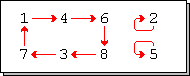
\includegraphics[scale=1.5]{cycle-1.png}
		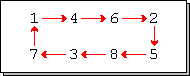
\includegraphics[scale=1.5]{cycle-2.png}
		\caption{This is a depiction of two elements thought of as elements of $S_8$. The first corresponds the the permutation fixing $2$ and $5$,
			and sending $1 \mapsto 4, 4 \mapsto 6, 6 \mapsto 8, 8\mapsto 3, 3 \mapsto 7, 7\mapsto 1$.
			The corresponding cycle notation for the first picture is $(146837)(2)(5)$ (where each parenthesized group of numbers
			correspond to a cycle in the above diagram). Similarly, the second permutation has cycle notation $(14625837)$.}

		\label{figure:cycle-notation}\end{figure}
\end{exercise}
\begin{remark}
	\label{remark:}
	If $s \in S_n$ is an element with certain cycle notation, we often omit all singletons from the cycle notation.
	So, for example, we denote the element of $S_8$ with cycle notation $(146837)(2)(5)$ simply as $(146837)$.
\end{remark}

You may prove the following facts, or assume them if you'd like:
\begin{fact}
	\label{fact:transpositions}
	\begin{enumerate}
		\item The symmetric group is generated by elements with cycle notation of the form $(ij)$. These elements are called {\bf transpositions}. That is, transpositions switch (transpose) two numbers in $\left\{ 1, \ldots, n \right\}$ and preserve the rest.
		\item If a group is generated by a collections of elements, the commutator subgroup is generated by commutators of those elements.
	\end{enumerate}
\end{fact}
\begin{exercise}
	\label{exercise:commutators-generate}
	Using \autoref{fact:transpositions}, show that $A_n$ is generated by commutators of transpositions.
\end{exercise}

\begin{exercise}
	\label{exercise:}
	Compute $A_4$ as a subgroup of $S_4$ in the following steps:
	\begin{enumerate}
		\item Show that $(123)(4)$ is the commutator of $(12)$ (the transposition switching $1$ and $2$) and $(13)$.
		\item Show that in general, the commutator of two transpositions is either a $3$-cycle when the transpositions have one element in common
		      (i.e., an element with cycle notation of the form $(abc)$
		      for $a,b,c \in \left\{ 1,2,3,4 \right\}$ distinct integers) or it is the identity permutation.
		\item Conclude from \autoref{exercise:commutators-generate} that $3$-cycles generate $A_4$.
		\item Compute the set of elements in $A_4$. Show it has size $12$.
		      \hint{You should get that $A_4$ contains all three cycles, together with the four elements $\id, (12)(34), (13)(24), (14)(23)$.}
	\end{enumerate}
\end{exercise}
\begin{exercise}
	\label{exercise:klein-4-commutator}
	Compute the commutator $\left[ A_4, A_4 \right]$. Show it has order $4$ and is explicitly given by the elements $\id, (12)(34), (13)(24), (14)(23)$.
	This is the Klein-$4$ group.
\end{exercise}

\newpage
\section{Commutators of $S_n$ and $A_n$}
\label{appendix:alternating}

For this appendix, we assume you have already read \autoref{appendix:commutators-s4}. In particular, we assume you are familiar with cycle notation
and the notion of transpositions.
The purpose of this appendix is to show $A_n$ is its own commutator for $n \geq 5$.
We do this in two subsections. In the first subsection, we give an alternate definition of $A_n$, and show that this agrees with the previous
definition \autoref{definition:alternating}. In the second section, we show $\left[ A_n, A_n \right] = A_n$ for $n \geq 5$.

\subsection{Equivalence of two definitions of $A_n$}

In this subsection, we give an alternate definition of $A_n$, from which it will be easier to show $\left[ A_n, A_n \right] = A_n$ for $n \geq 5$.
Recall above we defined the alternating group $A_n$ as the commutator $[S_n, S_n]$. For the purposes of this appendix,
we make the following alternate definition, and then verify $A_n$ is in fact $[S_n,S_n].$

\begin{definition}[Separate definition for this appendix]
	\label{definition:alternating-group-2}
	The {\bf alternating group}, $A_n$, is the subgroup of $S_n$ consisting of all elements $g \in S_n$ that can be written as a product of
	an even number of transpositions.
\end{definition}
\begin{exercise}
	\label{exercise:}
	Verify that the definition of $A_n$, \autoref{definition:alternating-group-2}, is well defined by showing that $A_n$ is in fact a subgroup.
\end{exercise}
\begin{exercise}
	\label{exercise:}**
	Suppose $g\in S_n$ can be written as products of transpositions in two ways, say $g = t_1 \cdots t_n$ and $g = r_1 \cdots r_m$ for $t_i, r_j$
	transpositions. Show $n \equiv m \bmod 2$.
	\hint{This is a bit tricky, and there are many ways to do it. Here is one nice one:
		Let $\sigma \in S_n$ be some permutation.
		Draw a picture with $1, 2, \cdots, n$ listed at the top and the bottom. Draw curves connecting $i$ to $\sigma(i)$ so that
		the lines always intersect transversely (i.e., no two curves are tangent at an intersection point).
		Check that the number of intersections of lines is well defined modulo $2$.
		Using that this number of intersections is well defined $\bmod 2$, check that
		the parity of the number of intersections agrees with the parity of the number of transpositions.
		Use this to conclude.}
\end{exercise}
\begin{exercise}
	\label{exercise:}
	Show that $\# A_n = \# S_n / 2 = n!/2$.
	\hint{Use \autoref{definition:alternating-group-2} to define a map $S_n \rightarrow C_2$ (where $C_2$ is the cyclic group of order $2$)
		so that $A_n$ is the set of elements mapping to the identity.}
\end{exercise}

\begin{exercise}
	\label{exercise:3-cycles}
	In this exercise, we show $A_n$ is generated by $3$-cycles.
	\begin{enumerate}
		\item Show that every $3$ cycle (i.e., a permutation written in cycle notation as $(ijk)$) lies in $A_n$.
		\item Show that every element in $A_n$ is a product of $3$-cycles. \hint{Show that if $i,j,k,l$ are distinct then $(ij)(kl)$ can be expressed as a product of two $3$-cycles. Then, expand any element as a product of transpositions and express any pair of transpositions as a product of one or two $3$-cycles.}
		\item Conclude $A_n$ is generated by $3$-cycles.
	\end{enumerate}
\end{exercise}

\begin{exercise}
	\label{exercise:}
	In this exercise, we check $\left[ S_n, S_n \right] = A_n$.
	\begin{enumerate}
		\item Show that $\left[ S_n, S_n \right] \subset A_n$. \hint{Expand commutators as products of transpositions and count their parity.}
		\item Show every $3$-cycle is a commutator. \hint{Consider the commutator of two transpositions.}
		\item Use \autoref{exercise:3-cycles} to conclude that $\left[ S_n, S_n \right] = A_n$.
	\end{enumerate}
\end{exercise}

\subsection{Commutator of $A_n$}
We now use our new definition of $A_n$, \autoref{definition:alternating-group-2}, to prove $\left[ A_n, A_n \right] = A_n$ when $n \geq 5$.
The proof is surprisingly easy, given what we have shown so far.
We start with the following warm-up computation.
\begin{exercise}[Warm up]
	\label{exercise:A-5-3-cycles}
	Show that in $A_5$, the commutator of $(123)$ and $(345)$ is $(235)$. That is, check $(123)(345)(132)(354) = (235)$.
\end{exercise}

\begin{exercise}
	\label{exercise:3-cycles-in-commutator}
	If $n \geq 5$, check that every $3$-cycle can be expressed as a commutator of two $3$-cycles.
	\hint{Relabel the numbers from \autoref{exercise:A-5-3-cycles}.}
\end{exercise}

\begin{exercise}
	\label{exercise:}
	Show $\left[ A_n, A_n \right] = S_5$.
	\hint{Recall from \autoref{exercise:3-cycles} that $A_n$ is generated by $3$-cycles. Then use \autoref{exercise:3-cycles}.}
\end{exercise}



\newpage
\theendnotes
\end{document}
